\documentclass[../main.tex]{subfiles}
\graphicspath{{\subfix{../img/}}}
\newacronym
  {pren1}                % id
  {PREN 1}                % display name
  {Produktentwicklung 1}  % full acronym name
  
\newacronym
  {pren2}                % id
  {PREN 2}                % display name
  {Produktentwicklung 2}  % full acronym name

\newacronym
  {yaml}
  {YAML}
  {YAML Ain't Markup Language}

\newacronym
  {tof-sensor}
  {ToF-Sensor}
  {Time-of-Flight Sensor}

\newglossaryentry{h-brücke}{
    name={H-Brücke},
    description={
         Eine H-Brücke ist eine Schaltung, die es ermöglicht, einen Elektromotor in beide Richtungen zu betreiben, indem sie den Stromfluss durch den Motor umkehrt. Sie besteht aus vier Schaltern (meistens Transistoren oder MOSFETs), die in einer "H"-Form angeordnet sind. Die Schalter werden so gesteuert, dass der Motor entweder vorwärts, rückwärts oder gestoppt wird.
    }
}


\newglossaryentry{pwm}{
    name={PWM},
    description={
        PWM (Pulsweitenmodulation) ist eine Technik zur Steuerung der Leistung von elektrischen Geräten, wie Motoren oder LEDs, durch das schnelle Ein- und Ausschalten eines Signals. Dabei wird die Dauer, in der das Signal "ein" ist (die Pulsbreite), im Vergleich zur Gesamtdauer eines Zyklus (der Periode) variiert.
    }
}


\newglossaryentry{ir-fototransistor}{
    name={IR-Fototransistor},
    description={
        Ein Fototransistor ist ein Halbleiterbauteil, das Licht in elektrischen Strom umwandelt. Wenn Licht auf den Transistor trifft, verändert sich seine elektrische Leitfähigkeit, was zu einer Stromänderung führt. Ein Infrarot(IR)-Fototransistor reagiert speziell auf Infrarotlicht. 
    }
}


\newglossaryentry{i2c}{
    name={I\textsuperscript{2}C},
    description={
        Eine serielle Kommunikationsschnittstelle, die den Datenaustausch zwischen verschiedenen Komponenten wie Mikrocontrollern, Sensoren und Aktoren über nur zwei Leitungen ermöglicht: \textit{Serial Data Line} für die Datenübertragung und \textit{Serial Clock Line} für die Synchronisation. 
        Die I\textsuperscript{2}C-Schnittstelle unterstützt mehrere Geräte in einem Netzwerk und verwendet Adressen, um einzelne Komponenten anzusprechen.
    }
}


\newglossaryentry{uart}{
    name={UART},
    description={
        Abkürzung für \textit{Universal Asynchronous Receiver Transmitter}. 
        Eine Hardware-Komponente oder ein Kommunikationsprotokoll, das zur seriellen, asynchronen Datenübertragung verwendet wird. 
        UART ermöglicht die Kommunikation zwischen zwei Geräten, indem Daten über eine Sendeleitung (\textit{TX}) und eine Empfangsleitung (\textit{RX}) übertragen werden. Es erfordert keine gemeinsame Taktleitung und verwendet stattdessen Start- und Stoppbits zur Synchronisation. 
    }
}


\newglossaryentry{PLA}{
    name={PLA},
    description={
    Polymilchsäure   (PLA) ist ein biologisch   abbaubarer, thermoplastischer Kunststoff, der aus erneuerbaren Ressourcen wie Maisstärke oder Zuckerrohr hergestellt wird.
    }}

\begin{document}

\newpage
\section{Lösungskonzept}\label{lösungskonzept}

In diesem Kapitel wird das gewählte Lösungskonzept ''Simpel'' (siehe Anhang \ref{a3:loesungsvariante_Simpel}) näher erläutert. Wieso das Lösungskonzept ''Beweglich'' ausgeschieden ist, steht im Anhang \ref{a3:EntscheidLösungsvariante} beschrieben. Bei dem gewählten Konzept liegt der Schwerpunkt auf einer möglichst einfachen Lösung, da ein einfach konstruiertes System in der Regel robuster im Einsatz ist. In der Abbildung \ref{img:Konzept-Skizze_Fahrzeug} ist eine Skizze von dem gewählten Lösungskonzept zu sehen.

\begin{figure}[H]
\centering
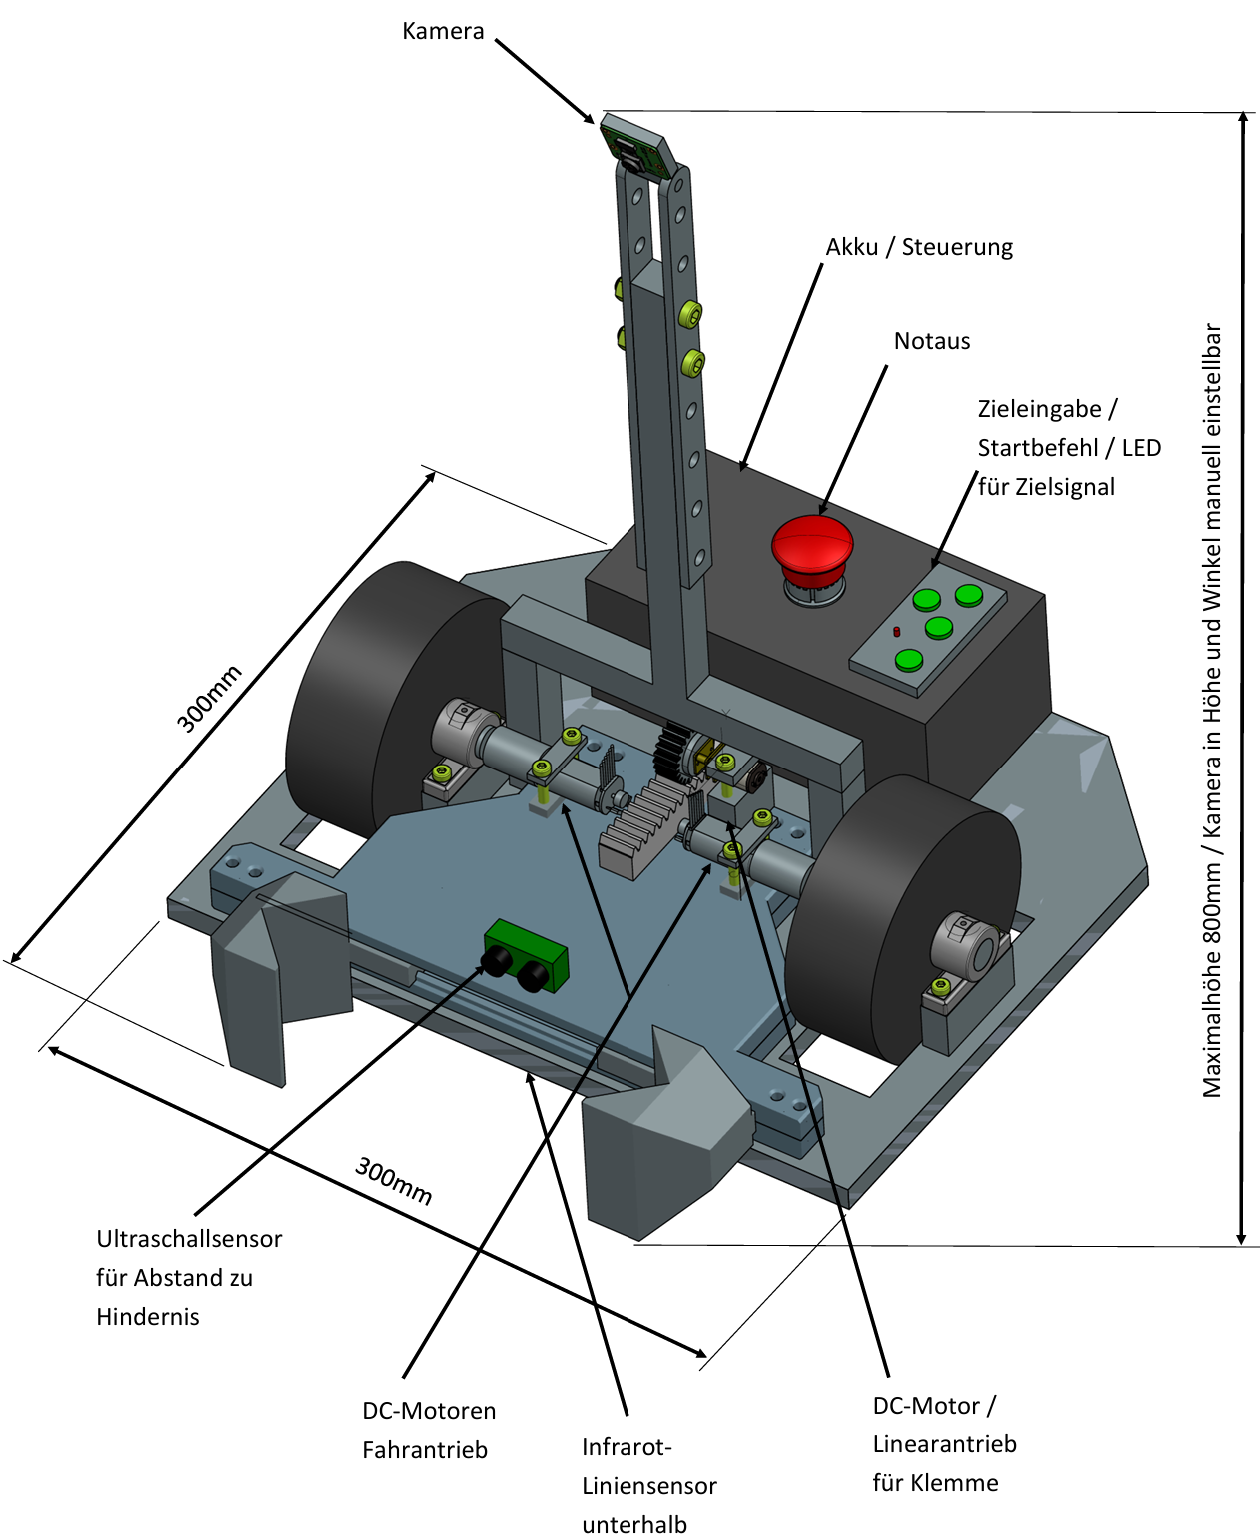
\includegraphics[width=0.85\linewidth]{Skizze Konzept beschriftet.png}
\caption{Skizze des Lösungskonzepts}
\label{img:Konzept-Skizze_Fahrzeug}
\end{figure}

\subsection{Aufbau}

Das Fahrzeug besitzt zwei Räder, die mit jeweils einem DC-Motor angetrieben werden. Um das Fahrzeug zu balancieren, hat es am hinteren Fahrzeugende eine dritte Auflagefläche.

Die Raspberry Pi Module 3 Kamera befindet sich auf einem höhenverstellbaren Masten. Die Höhe der Kamera kann zwischen 40 und 60 Zentimeter manuell eingestellt werden. Der Winkel der Kamera kann ebenfalls manuell verändert werden. Somit kann die Kamera-Position im späteren Verlauf des Projektes einfach optimiert werden.

Zur Hindernisbewältigung befindet sich an der Vorderseite des Fahrzeugs ein Klemmmechanismus. Ein dritter DC-Motor zieht die beiden Klemmbacken des Mechanismus zusammen und hebt sie an, um das Hindernis aufzuheben. Damit der Abstand zu einem Hindernis erkannt werden kann, befindet sich ein Ultraschallsensor zwischen den beiden Klemmbacken. 

Die Motoren und Sensoren werden über das TinyK22 gesteuert.
Das TinyK22, die Eingabeknöpfe sowie die Kamera sind an einem Raspberry Pi 5 angeschlossen.

Ein LiPo-Akku stellt die Energieversorgung sicher(Begründung im Anhang \ref{a3:Energiequelle}).
Mit dem Notaus-Knopf kann die Energieversorgung zu allen Komponenten direkt unterbrochen werden.
\newline
\newline
\begin{figure}[H]
\centering
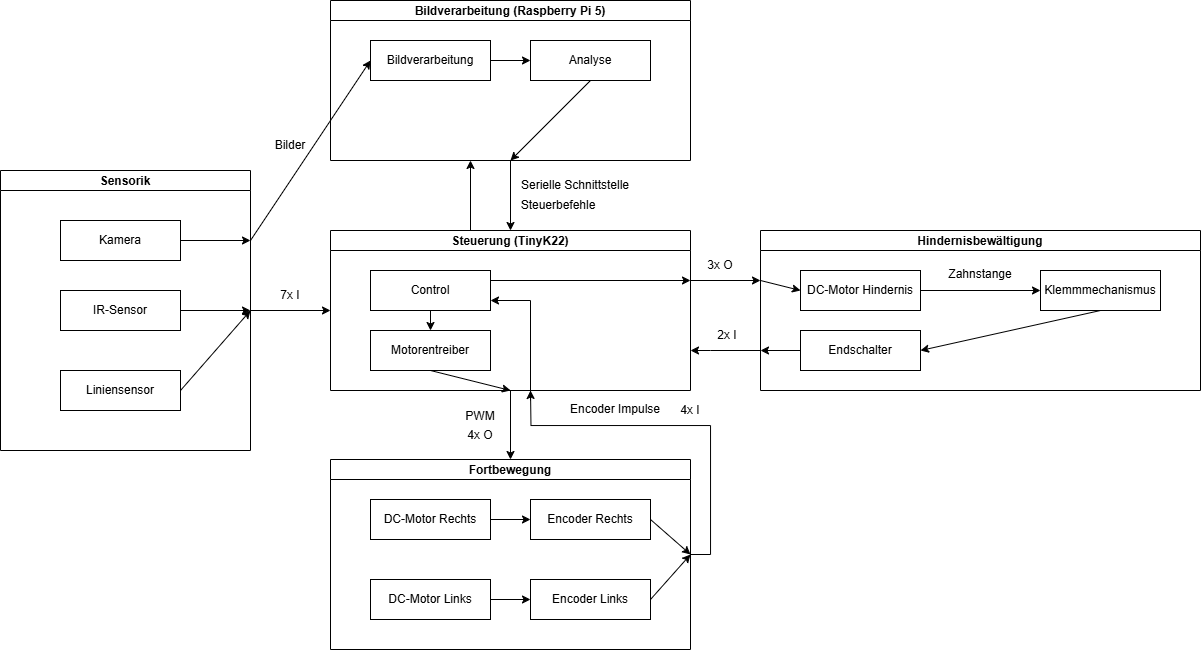
\includegraphics[width=1\textwidth]{img/lösungskonzpet/Blockschaltbild.png}
\caption{Blockschaltbild Aufbau}
\label{img:Blockschaltbild-Aufbau}
\end{figure}

{\color{red} TODO(Feedback Gian) zu Blockschaltbild:} \\
- Sehr klein, entweder versuchen Schriftgrösse zu erhöhen oder in Landscape mode \\
- TinyK22 sendet Informationen (Gefahrener Weg, Genauer Winkel bei Drehung, Fehlende Linie) an RaspberryPi \\

\newpage
\subsection{Ablauf}

Im Ablaufdiagramm (Abbildung \ref{img:ablaufdiagramm}) wird der Programmablauf des Fahrzeugs von Start bis Ziel übersichtlich aufgezeigt.

\begin{figure}[H]
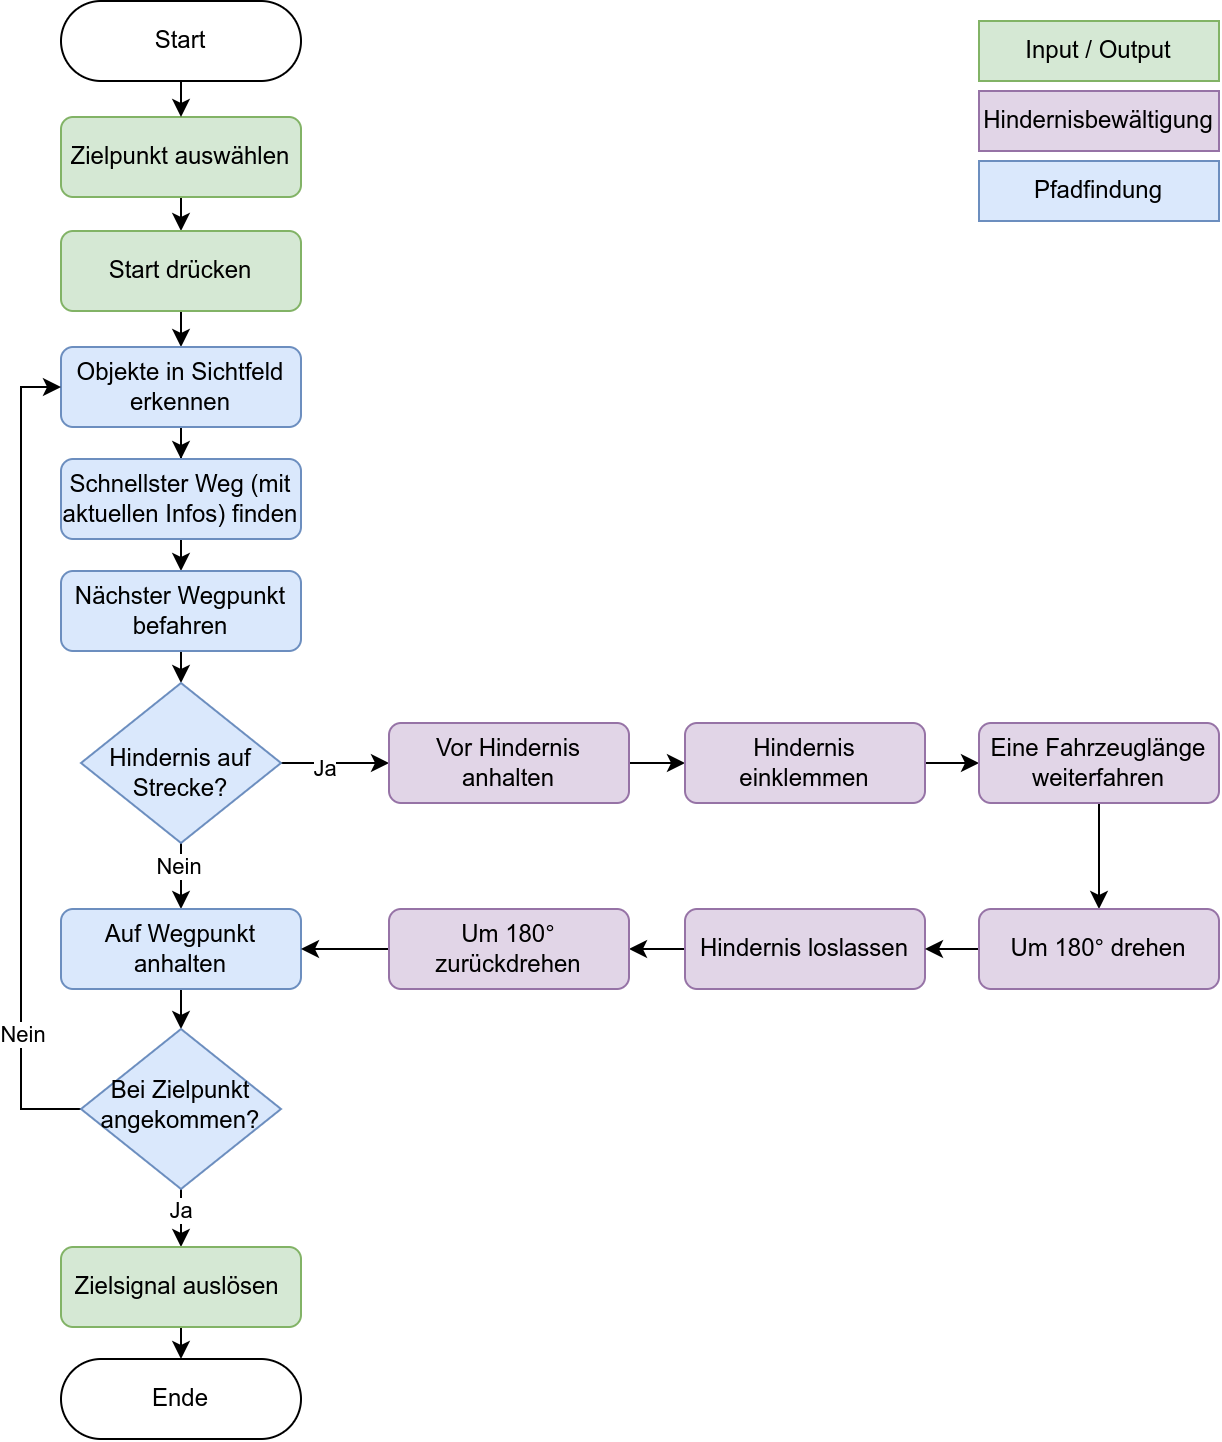
\includegraphics[width=0.9\textwidth]{img/lösungskonzpet/Ablaufdiagramm.png}
\caption{Ablaufdiagramm}
\label{img:ablaufdiagramm}
\end{figure}

\newpage
\subsection{Zielauswahl}
\imagefloat{img/lösungskonzpet/Skizzen/Zielauswahl.png}{Zielauswahl (Ausschnitt aus Abbildung \ref{img:Konzept-Skizze_Fahrzeug})}{0.3\textwidth}

Das Ziel des Fahrzeugs muss vor dem Start ausgewählt werden. Die Auswahlmöglichkeiten sind A, B oder C. Jede dieser Optionen kann über einen physischen Knopf am Fahrzeug festgelegt werden.

Neben der Zielauswahl befindet sich der Knopf zum Starten des Fahrzeugs. Dieser funktioniert erst, wenn ein Ziel ausgewählt wurde. Bei einer mehrfachen Zielauswahl wird das zuletzt gewählte Ziel angesteuert.

Sobald das Fahrzeug das Ziel erreicht hat, leuchtet die LED neben der Starttaste auf.

\subsection{Fortbewegung} 

Die Fortbewegung wird nach dem Prinzip Roomba realisiert: zwei einzeln angetriebene Räder mit einem Stützelement. Es handelt sich dabei um ein ähnliches System, wie es bei Staubsauger-Robotern vorkommt. Die angetriebenen Räder können unabhängig in beide Drehrichtungen angetrieben werden, wodurch ein Wenden an Ort und Stelle ermöglicht wird. Die beiden Räder sind in Längsrichtung zentrisch angeordnet, damit sich das Fahrzeug um den eigenen Mittelpunkt drehen kann, ohne dass ein Versatz entsteht. Weitere Details dazu befinden sich im Anhang unter \ref{a3:Fortbewegung}.

Als Antriebsmotoren werden DC-Motoren verwendet, die als Motorentreiber eine \gls{h-brücke} verwenden. Diese wird für die Geschwindigkeit mit einem \gls{pwm}-Signal angesteuert. Jeder Motor verfügt über einen Encoder, der überwacht, dass beide Motoren die gleiche Anzahl an Umdrehungen ausführen können. Gesteuert werden die Motoren von einem TinyK22 (wieso der TinyK22 gewählt wurde, siehe Anhang \ref{a3:Hardware Steuerung}), der die \gls{h-brücke} ansteuert. Weitere Details können im Anhang, unter \ref{a3:Fahrantrieb} (Fahrantrieb) und \ref{a3:Sensorik:Positionsabfrage} (Sensorik Positionsabfrage) nachgeschlagen werden.
\newpage
Der TinyK22 ist über eine \Gls{uart}-Schnittstelle mit dem Raspberry Pi verbunden (siehe Abbildung \ref{img:UART_Physisch}). Der Raspberry Pi analysiert mit der Kamera den nächstbesten Punkt ohne Pylone. Anschliessend teilt er dem TinyK22 mit, um welchen Winkel das Fahrzeug ausgerichtet werden muss. Somit dreht sich das Fahrzeug auf die angepeilte Linie, die vom Liniensensor erkannt wird. Wird die Linie nicht erkannt, sucht das System diese durch Drehungen im Bereich von ±15 Grad. Sobald die Linie gefunden wird, meldet der TinyK22 dem Raspberry Pi, wie weit sich das Fahrzeug gedreht hat. Dies ist in der Abbildung \ref{img:UART_Signalablauf} visualisiert.

\begin{figure}[H]
\centering
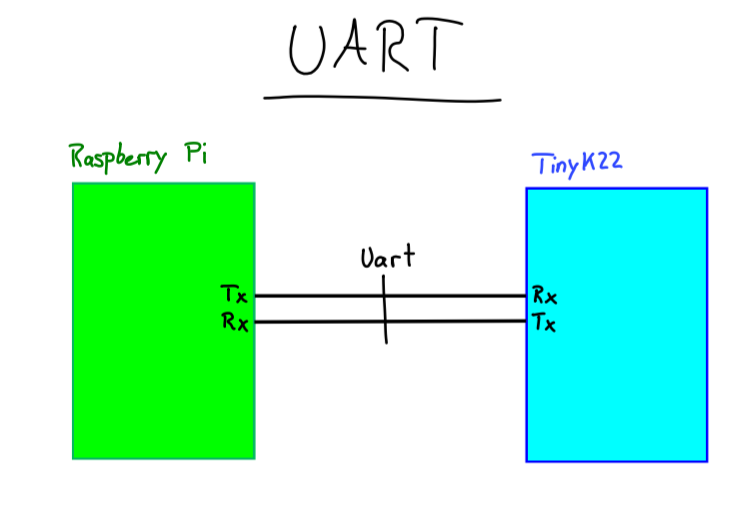
\includegraphics[width=0.6\textwidth]{img/lösungskonzpet/Skizzen/Uart_Physisch.png}
\caption{\Gls{uart} Physische Verbindung}
\label{img:UART_Physisch}
\end{figure}

\begin{figure}[H]
\centering
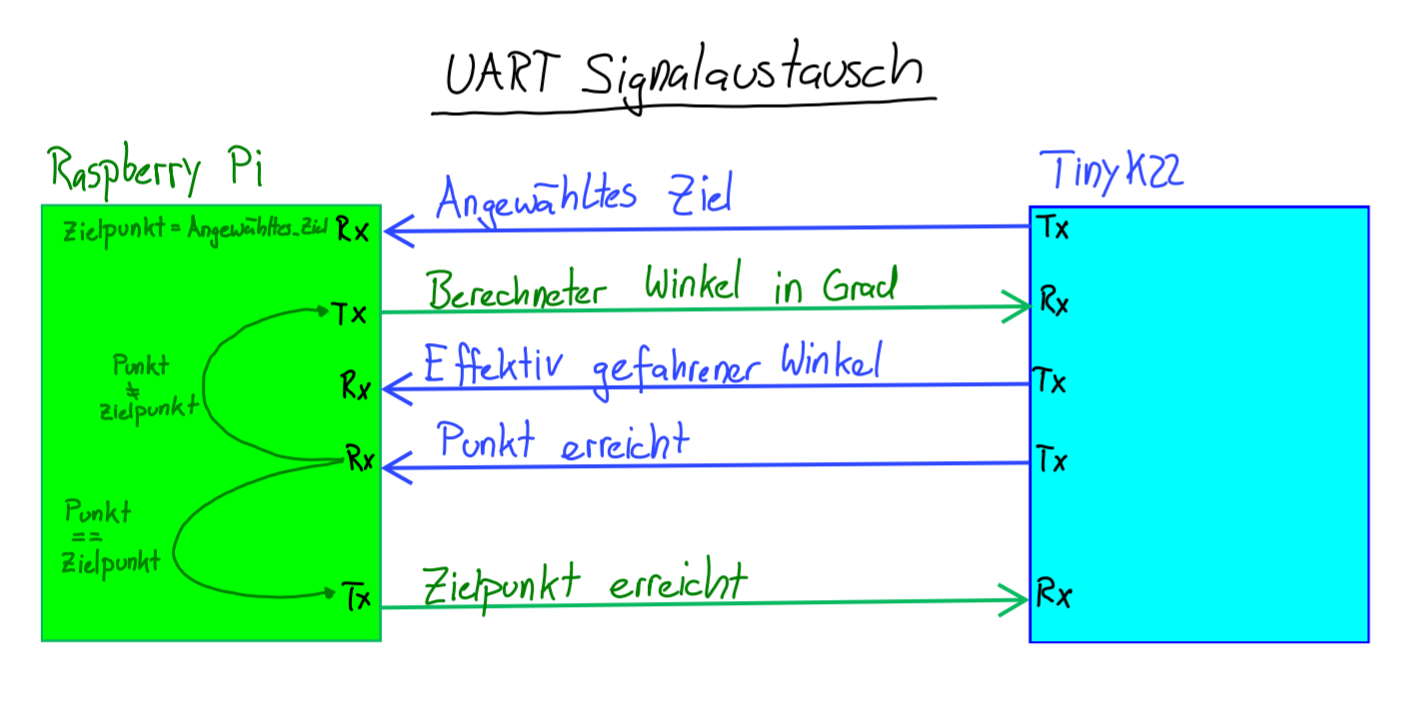
\includegraphics[width=0.8\textwidth]{img/lösungskonzpet/Skizzen/Uart_Signalaustausch.png}
\caption{\Gls{uart} Signalablauf}
\label{img:UART_Signalablauf}
\end{figure}


Das Fahrzeug folgt der Linie mithilfe des Liniensensors. Erkennt der Sensor eine breitere Linie, also einen Punkt, informiert der TinyK22 den Raspberry Pi, stoppt das Fahrzeug, und der Vorgang beginnt erneut. Sobald das Fahrzeug den Zielpunkt erreicht, signalisiert der Raspberry Pi dies dem TinyK22. Der TinyK22 lässt anschliessend die LED blinken.

\newpage

\subsection{Wegfindung}

Der schnellste Weg ins Ziel wird, wie in der Konzeptfindung festgelegt (siehe Anhang \ref{a3:Wegfindung}), mithilfe des Dijkstra-Algorithmus berechnet. Dabei wird das vorgegebene Liniennetz als gewichteter Graph in der Software gespeichert. Ursprünglich besitzen alle Kanten eine einheitliche Gewichtung. Sobald die Kamera neue Informationen über die Strecke erfasst (siehe \ref{sub:Objekterkennung}), wird der Graph entsprechend aktualisiert, und der kürzeste Weg wird basierend auf der aktuellen Position neu berechnet.

Je nach neu erhaltener Information werden folgende Anpassungen am Graphen vorgenommen: \begin{itemize} 
  \item Pylon auf Wegpunkt erkannt: Der Wegpunkt (Knoten) wird aus dem Graphen entfernt.
  \item Linie wurde entfernt: Die Linie (Kante) wird aus dem Graphen entfernt. 
  \item Hindernis auf Linie erkannt: Die Linie (Kante) erhält eine höhere Gewichtung.
\end{itemize}

\subsubsection{Objekterkennung} \label{sub:Objekterkennung}
Die weitwinklige Raspberry Pi Module 3 Kamera führt die Objekterkennung durch. Dabei werden Pylonen, Hindernisse und Wegpunkte erkannt. Als Software kommt YOLO zum Einsatz (Anhang \ref{a3:Objekterkennung}). Die erkannten Objekte werden für die Wegfindung genutzt. Das Ziel ist es, von Anfang an möglichst viele Objekte zu erfassen und auszuwerten. Da dies jedoch nicht garantiert werden kann, wird die Objekterkennung bei jedem Wegpunkt durchgeführt. 

\subsection{Hindernisbewältigung}
Der Ultraschallsensor überwacht kontinuierlich, ob sich ein Hindernis auf der Linie befindet (Sensorwahl: Anhang \ref{a3:Objekterkennung_Sensor}). Ab einer Entfernung von 30 cm wird ein Hindernis erkannt. Das Fahrzeug hält an, sobald das Hindernis sich zwischen den zwei seitlichen Klemmbacken befindet. Danach wird der DC-Motor angesteuert, der das Hindernis ergreift und gleichzeitig anhebt. Die genauen Details zu dieser Konstruktion befinden sich im Anhang \ref{a3:Hindernisbewältigungsantrieb} und \ref{a3:Aufnahme_Hindernis}.
Das Fahrzeug fährt anschliessend eine Fahrzeuglänge vor, wobei die Encodermessung die Distanz überwacht. Danach dreht es sich um 180 Grad, und der Motor löst die Klemmen. Das Fahrzeug entfernt sich nun so weit vom Hindernis, bis es sich ohne Kollisionsgefahr um 180 Grad zurückdrehen kann. Abschliessend fährt das Fahrzeug mithilfe des Liniensensors entlang der Linie zum nächsten Punkt (siehe Abbildung \ref{img:Skizze_Hindernisbewältigung}).

\begin{figure}[H]
\centering
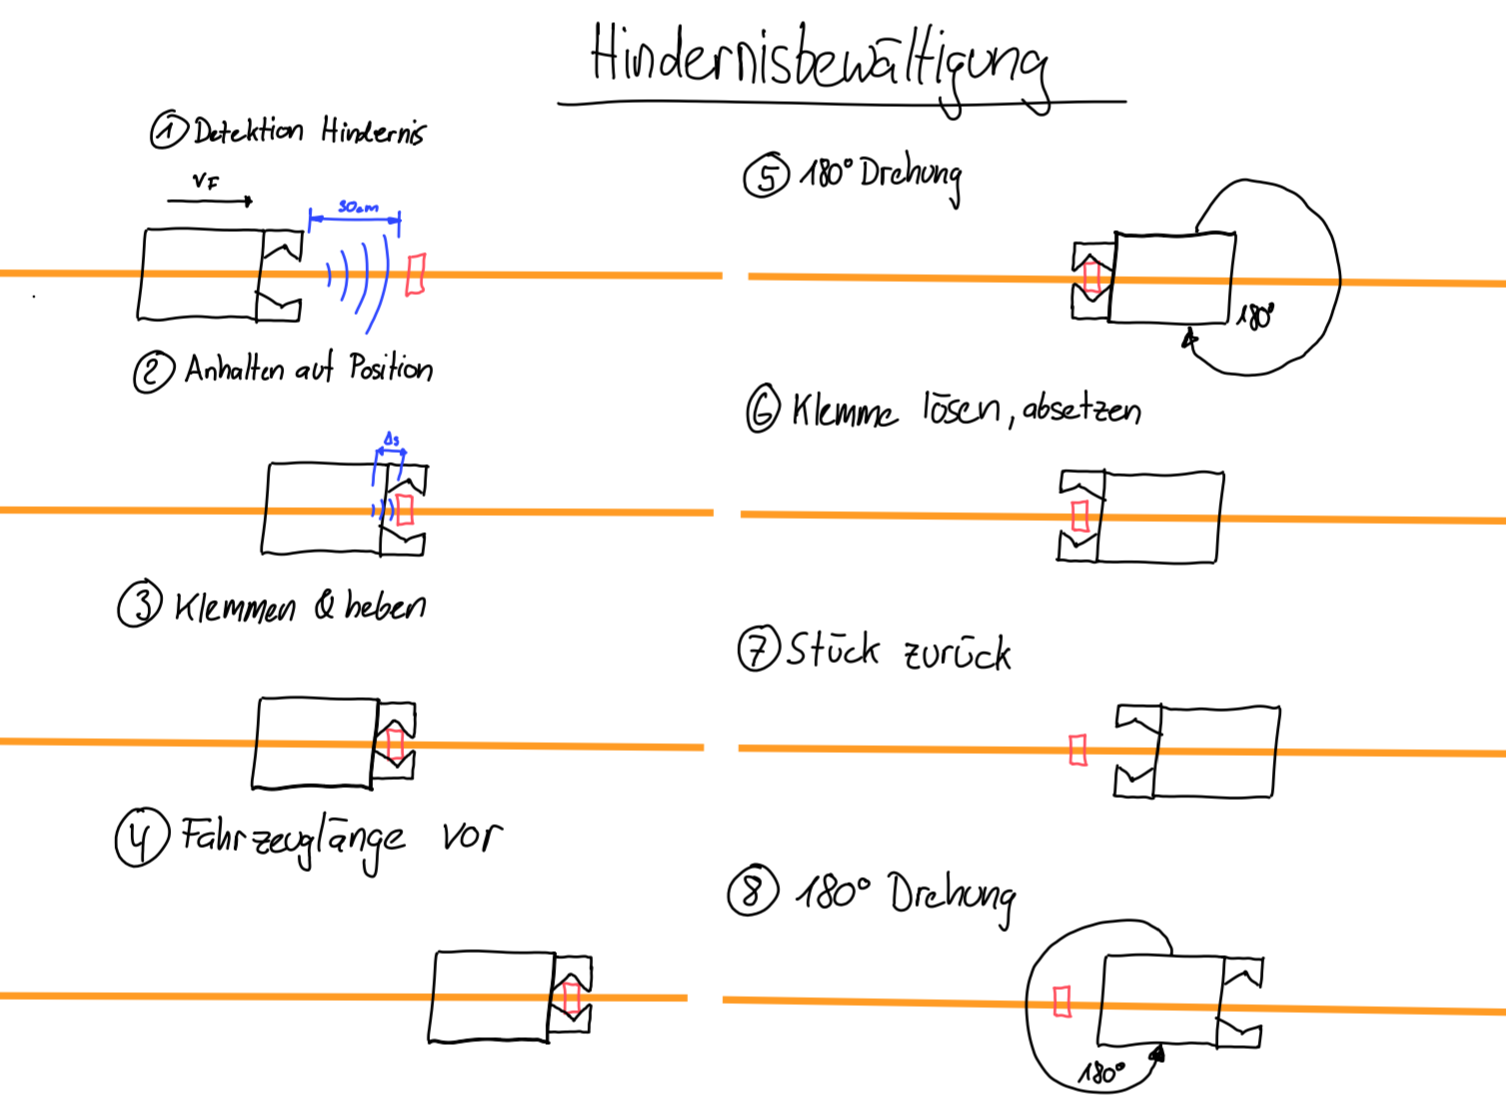
\includegraphics[width=0.8\textwidth]{img/lösungskonzpet/Skizzen/Skizze_Hindernisbewältigung.png}
\caption{Ablauf der Hindernisbewältigung}
\label{img:Skizze_Hindernisbewältigung}
\end{figure}


\subsubsection{Klemmmechanismus}
Der Klemmmechanismus, welcher in Punkt 3 und 6 in der Abbildung \ref{img:Skizze_Hindernisbewältigung} benötigt wird, erfüllt mehrere Funktionen.

\begin{enumerate}
    \item Greifen
    \item Anheben
    \item Senken
    \item Loslassen
\end{enumerate}

Alle Funktionen werden mithilfe eines DC-Motors ausgeübt. Das Design ist in Abbildungen \ref{fig:greifarm_oben} und \ref{fig:greifarm_unten} ersichtlich.
\newline

Zusätzlich soll die Konstruktion helfen, Fehler bei der Messung auszukorrigieren.
\begin{enumerate}
    \item Korrektur Winkel (bis zu 15°, siehe Rechnung für Design in Anhang \ref{loes:winkel_verschiebung})
    \item Korrektur Distanz (bis zu 2.25 cm, siehe Rechnung für Design in Anhang \ref{loes:winkel_verschiebung})
    \item Korrektur Offset (bis zu 2 cm, siehe Definition für Design in Anhang \ref{loes:abstand_klemmen})
\end{enumerate}

\begin{figure}[h!]
    \centering
    % Erste Minipage für das obere Bild
    \begin{minipage}[t]{0.45\textwidth}
        \centering
        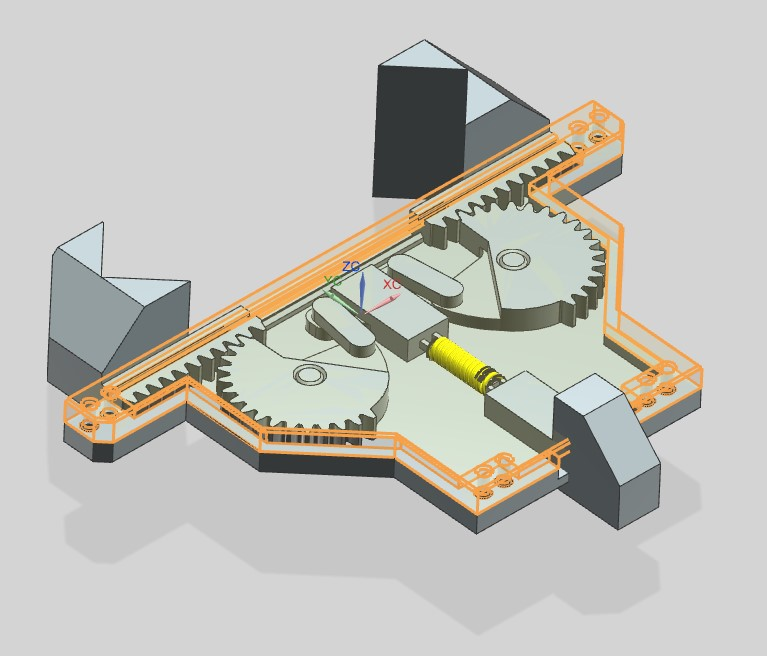
\includegraphics[height=6cm]{img/lösungskonzpet/hindernissaufnahme/Greifarm_oben.jpg}
        \caption{Klemm- \& Hebemechanismus von oben}
        \label{fig:greifarm_oben}
    \end{minipage}
    \hfill
    % Zweite Minipage für das untere Bild
    \begin{minipage}[t]{0.45\textwidth}
        \centering
        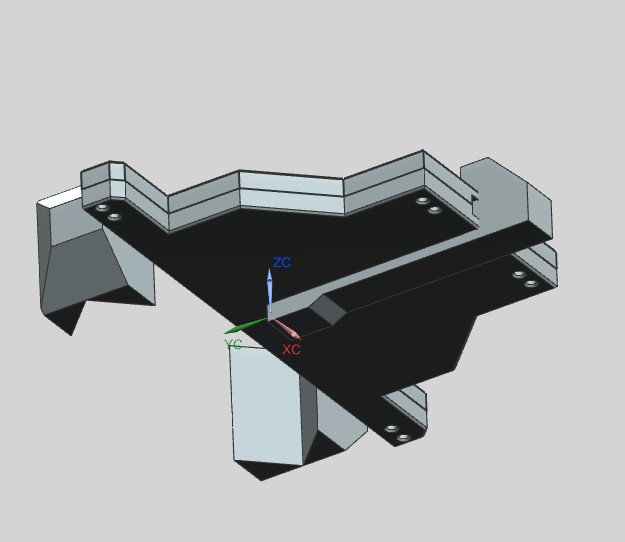
\includegraphics[height=6cm]{img/lösungskonzpet/hindernissaufnahme/Greifarm_unten.jpg}
        \caption{Klemm- \& Hebemechanismus von unten}
        \label{fig:greifarm_unten}
    \end{minipage}
\end{figure}
\newpage
Abbildung \ref{fig:greifarm_oben} zeigt den Klemmmechanismus. Er wird durch Zahnräder angetrieben, welche wiederum von einem linearen Mechanismus bewegt werden, um gleichzeitig den Hebemechanismus auszulösen. Die Feder (Gelb in Abbildung \ref{fig:greifarm_oben} ersichtlich) sorgt dafür, dass, sobald die nötige Griffkraft erreicht ist, weiterhin eine Bewegung für den Hebemechanismus ermöglicht wird. In Abbildung \ref{fig:greifarm_unten} ist der Hebemechanismus zu sehen, der sich von einer Plattform (nicht im Bild sichtbar) abdrückt. An den Rändern befinden sich acht Löcher, von denen vier für Schrauben und die anderen vier für Führungen genutzt werden, um eine kontrollierte Anhebung des Hindernisses durch den Mechanismus sicherzustellen.
Der DC-Motor, der den gesamten Mechanismus antreibt, wäre am Gehäuse angebracht.
Der abgebildete Mechanismus wurde zu Testzwecken für die händische Bedienung ausgelegt. Die Tests des Mechanismus sind im Kapitel \ref{sec:hardware_greifarm} ersichtlich.

\subsection{Materialwahl}
Die Materialwahl für den Klemm- \& Hebemechanismus sowie das \enquote{Chassis} ist essenziell. Nicht nur, um die Funktion korrekt zu erfüllen, sondern vor allem, um Gewicht einzusparen. Aufgrund der Komplexität, der genauen Geometrie und geringer Belastungen, wurde für den Klemm- \& Hebemechanismus 3D-Druck ausgewählt. Wahrscheinlich wird PLA-Filament oder, wenn nötig, ein dauerfesteres Filament eingesetzt. Da das gesamte Gewicht der Komponenten auf dem Chassis liegt, wird Aluminium als Material verwendet. Holz hat eine viermal geringeren Dichte und könnte ebenfalls genutzt werden. Da jedoch die Erfahrungen im Team sowie die Ausstattung der Werkstatt auf Metalle ausgerichtet sind, wird vorläufig Aluminium verwendet. Die Wahl der Materialien wurde vorläufig definiert, muss jedoch zu einem späteren Zeitpunkt getestet werden.



\subsection{Prototyping Ergebnisse}
In diesem Kapitel werden die Ergebnisse verschiedener Tests kurz vorgestellt. Diese Ergebnisse sind entscheidend für das entstandene Lösungskonzept.
Die ausführlichen Berichte zu den durchgeführten Tests befinden sich im Kapitel Prototyping im Anhang \ref{a4 prototyping}.

\subsubsection{Klemm- \& Hebemachanismus} \label{sec:hardware_greifarm}
Damit das allgemeine Funktionsprinzip getestet und Verbesserungen am Klemm- und Hebemechanismus gemacht werden können, wurde ein Prototyp 3D - gedruckt (siehe Abbildung \ref{fig:hardware_test_fertig}). Bei dem Zusammenbau und Funktionalitätstests wurden diverse Erkenntnisse gewonnen:

\begin{enumerate}
    \item Funktionalität des Klemmmechanismus:
    \begin{itemize}
        \item Der Klemmmechanismus kann das Hindernis klemmen.
        \item Der Winkel für die Klemmbacken funktioniert einwandfrei.
        \item Die Führung der Klemmbacken muss vergrößert werden, da Schrumpfungseffekte durch 3D-Druck auftreten (siehe Abbildung \ref{fig:hardware_test_klemmen_gleiten}).
    \end{itemize}
    \item Platz- und Offset-Probleme:
    \begin{itemize}
        \item Zwischen den Klemmbacken ist nicht genügend Platz vorhanden, die Offset-Reserve fehlt.
    \end{itemize}
    \item Probleme mit dem Hebemechanismus:
    \begin{itemize}
        \item Der Hebemechanismus funktioniert nicht, da die Feder nicht geführt ist (siehe Abbildung \ref{fig:hardware_test_schieber}).
        \item Für die lineare Bewegung fehlt eine geeignete Führung.
    \end{itemize}
    \item Probleme mit Zahnrädern und Verbindungen:
    \begin{itemize}
        \item Zahnräder reiben an der Decke. Der Luftspalt zwischen Zahnrad und Deckel ist zu klein und muss vergrössert werden.
        \item Die Verbinder zwischen Schieber und Zahnrädern müssen verlängert werden.
    \end{itemize}
    \item Fertigungsprobleme:
    \begin{itemize}
        \item Alle Löcher sind zu klein aufgrund von Schrumpfungseffekten beim 3D-Druck (siehe Abbildung \ref{fig:hardware_test_loecher}).
    \end{itemize}
    \item Allgemeine Verbesserungsvorschläge:
    \begin{itemize}
        \item Für ein besseres Verhalten des gesamten Systems sollte Silikonspray verwendet werden.
    \end{itemize}
\end{enumerate}
\newpage
\begin{figure}[h!]
    \centering
    \begin{minipage}[t]{0.45\textwidth}
        \centering
        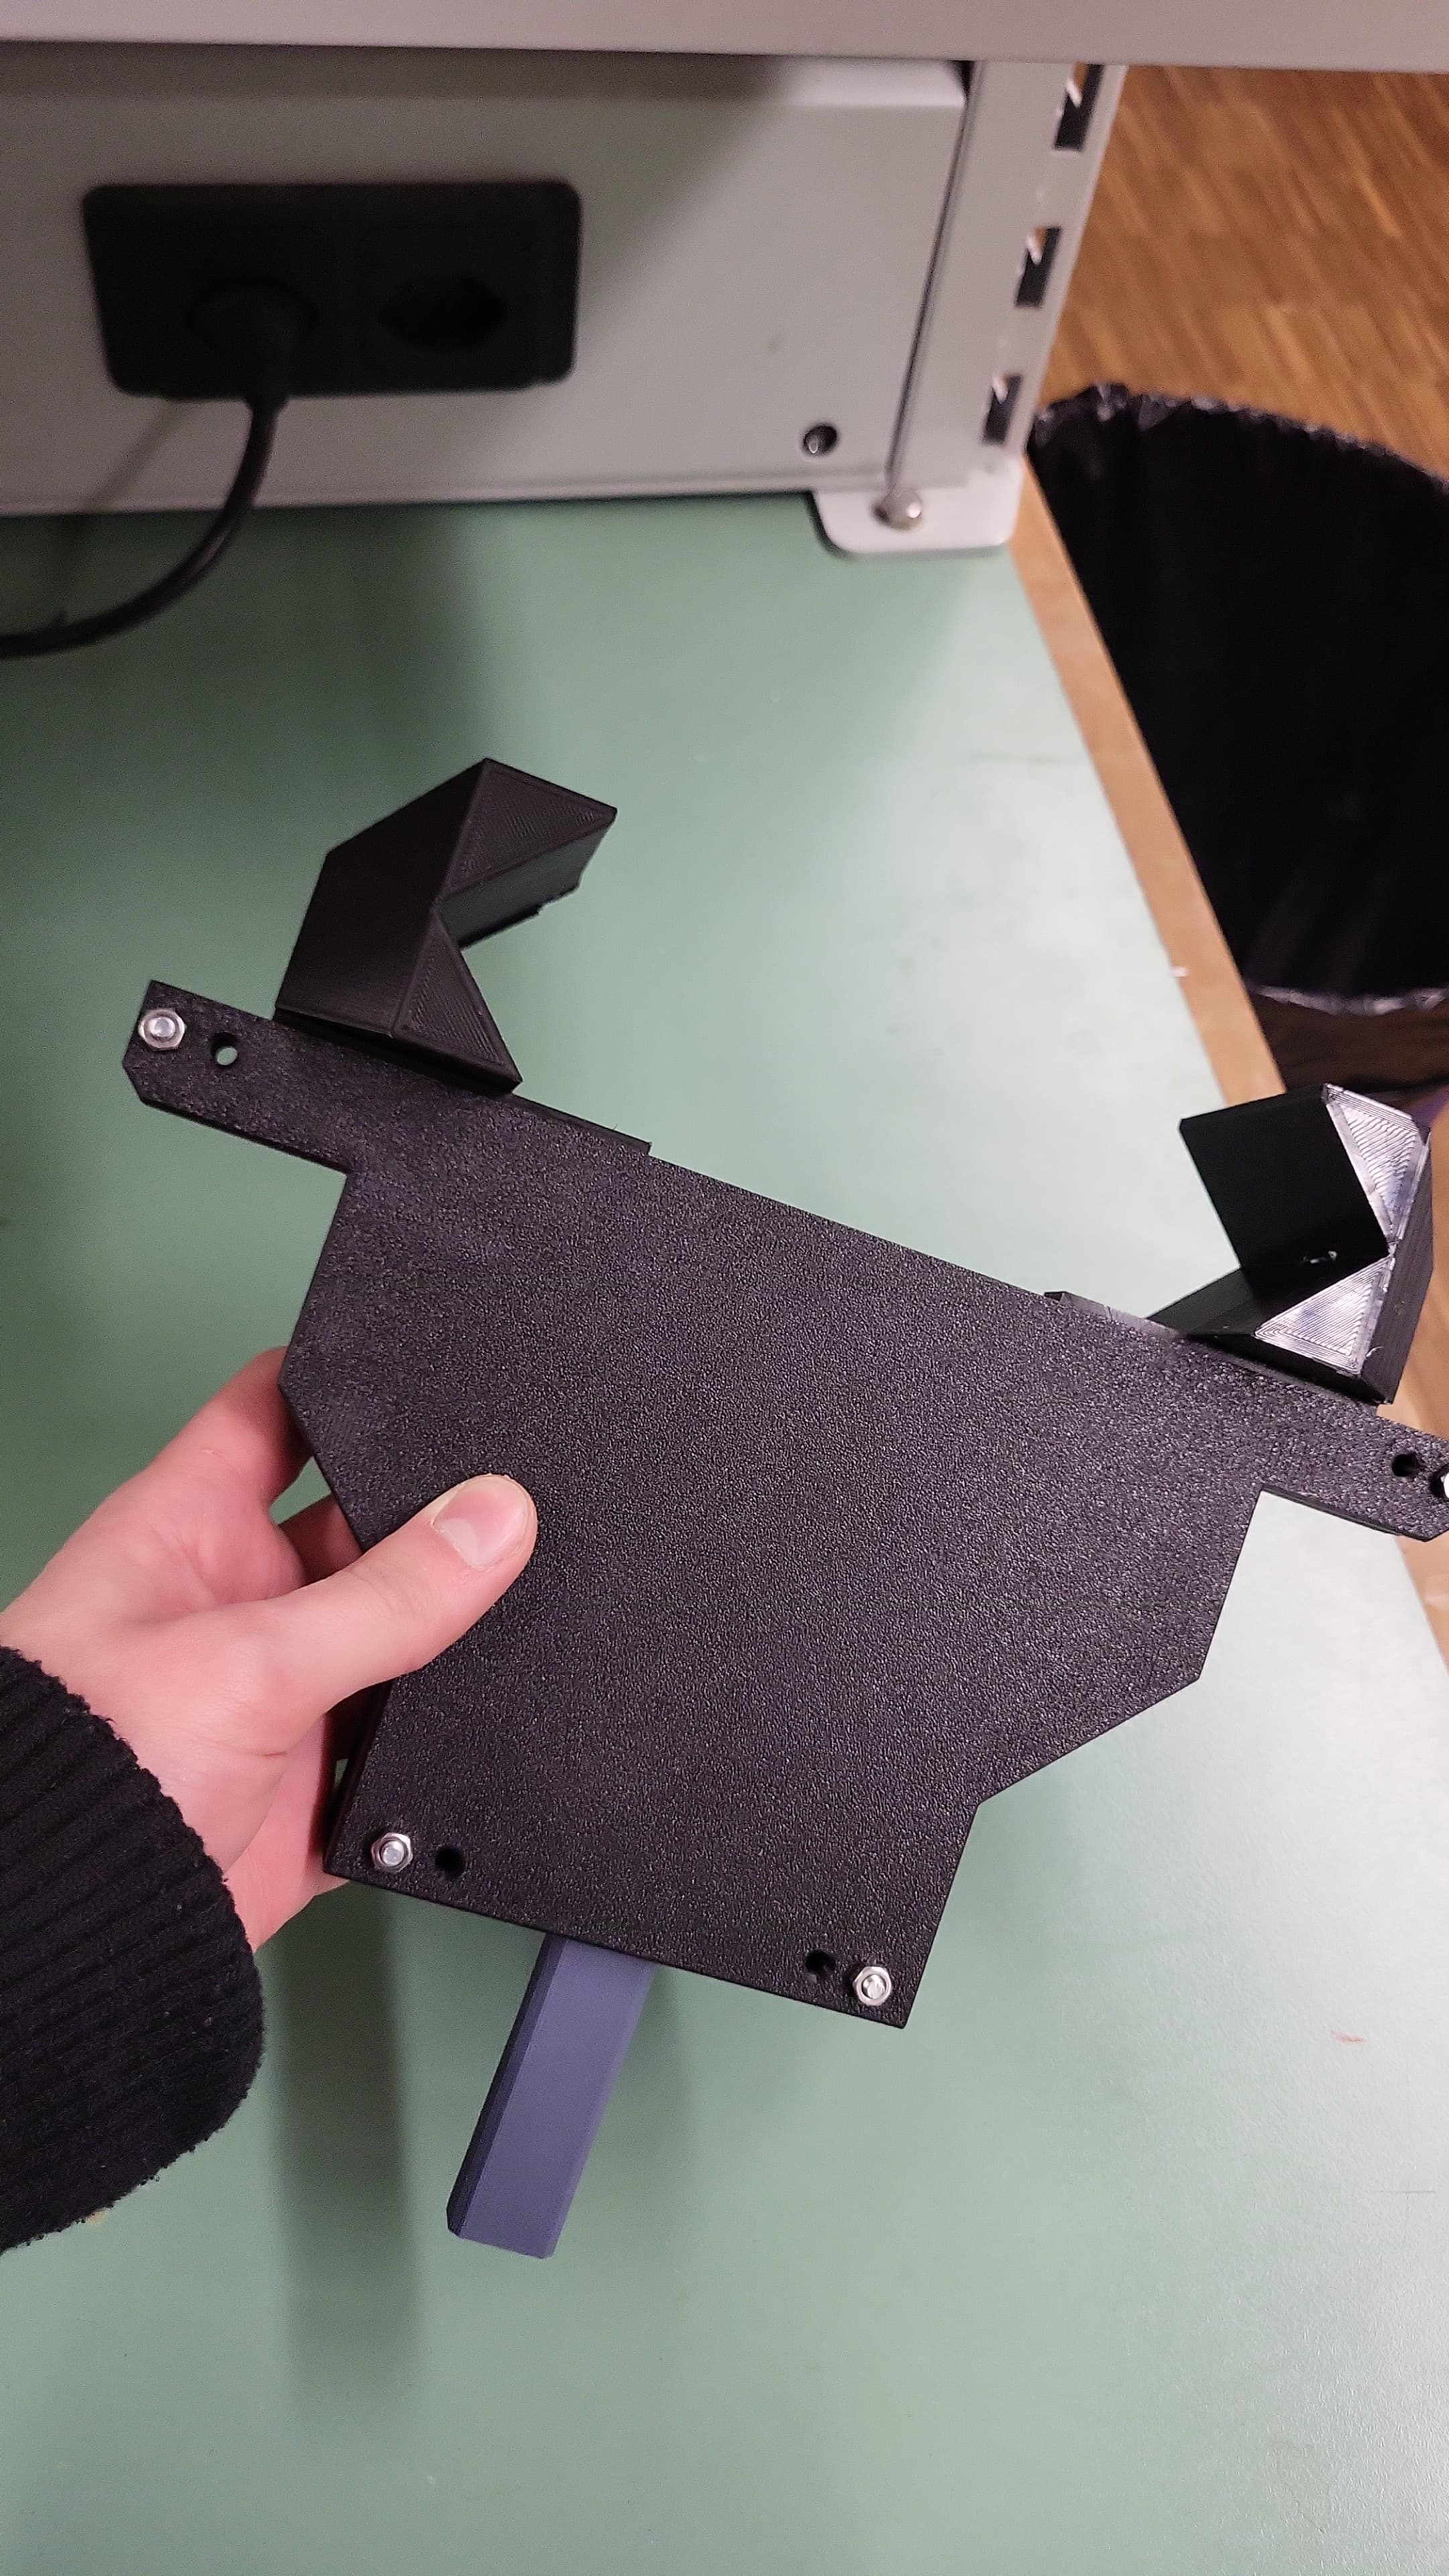
\includegraphics[height=9cm]{img/greifarmtest/prototyp_test_fertig.jpeg}
        \caption{Prototyp von Aussen}
        \label{fig:hardware_test_fertig}
    \end{minipage}%
    \hfill
    \begin{minipage}[t]{0.45\textwidth}
        \centering
        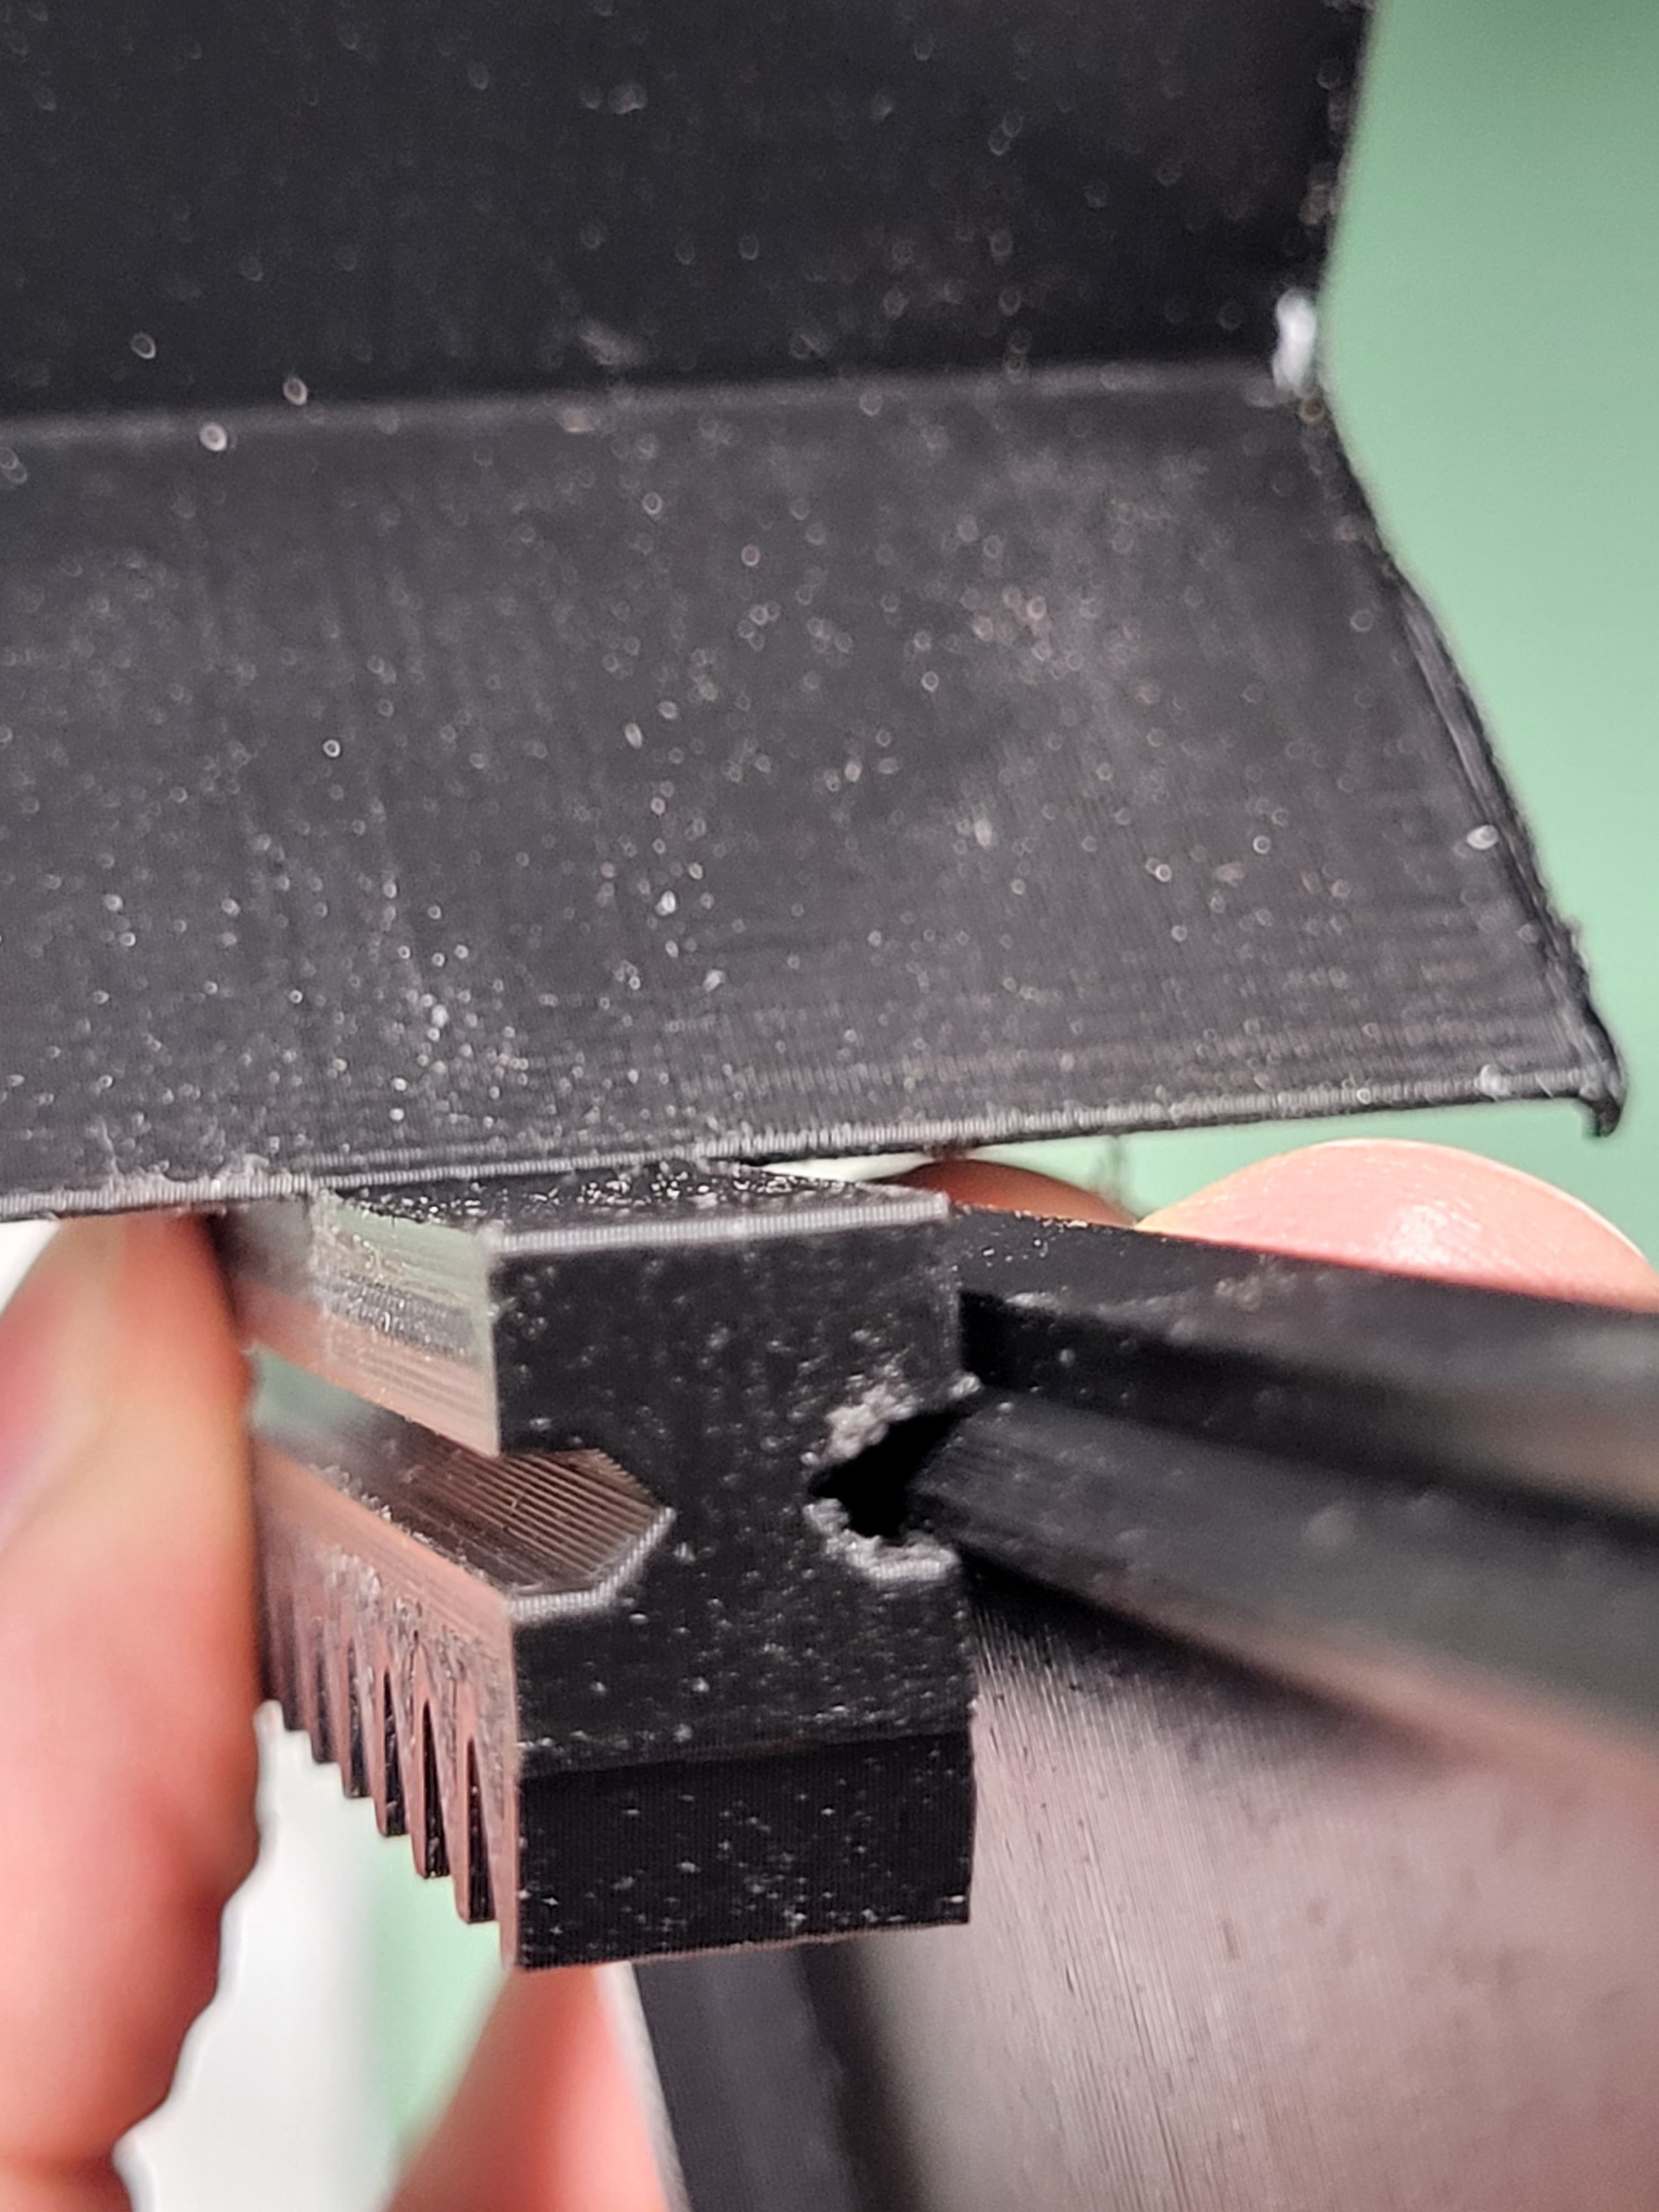
\includegraphics[height=9cm]{img/greifarmtest/prototyp_test_klemmen_gleiten.jpeg}
        \caption{Schrumpfungseffekte 3D-Druck: Führung der Klemmbacken passen nicht}
        \label{fig:hardware_test_klemmen_gleiten}
    \end{minipage}
\end{figure}

\begin{figure}[h!]
    \centering
    \begin{minipage}[t]{0.45\textwidth}
        \centering
        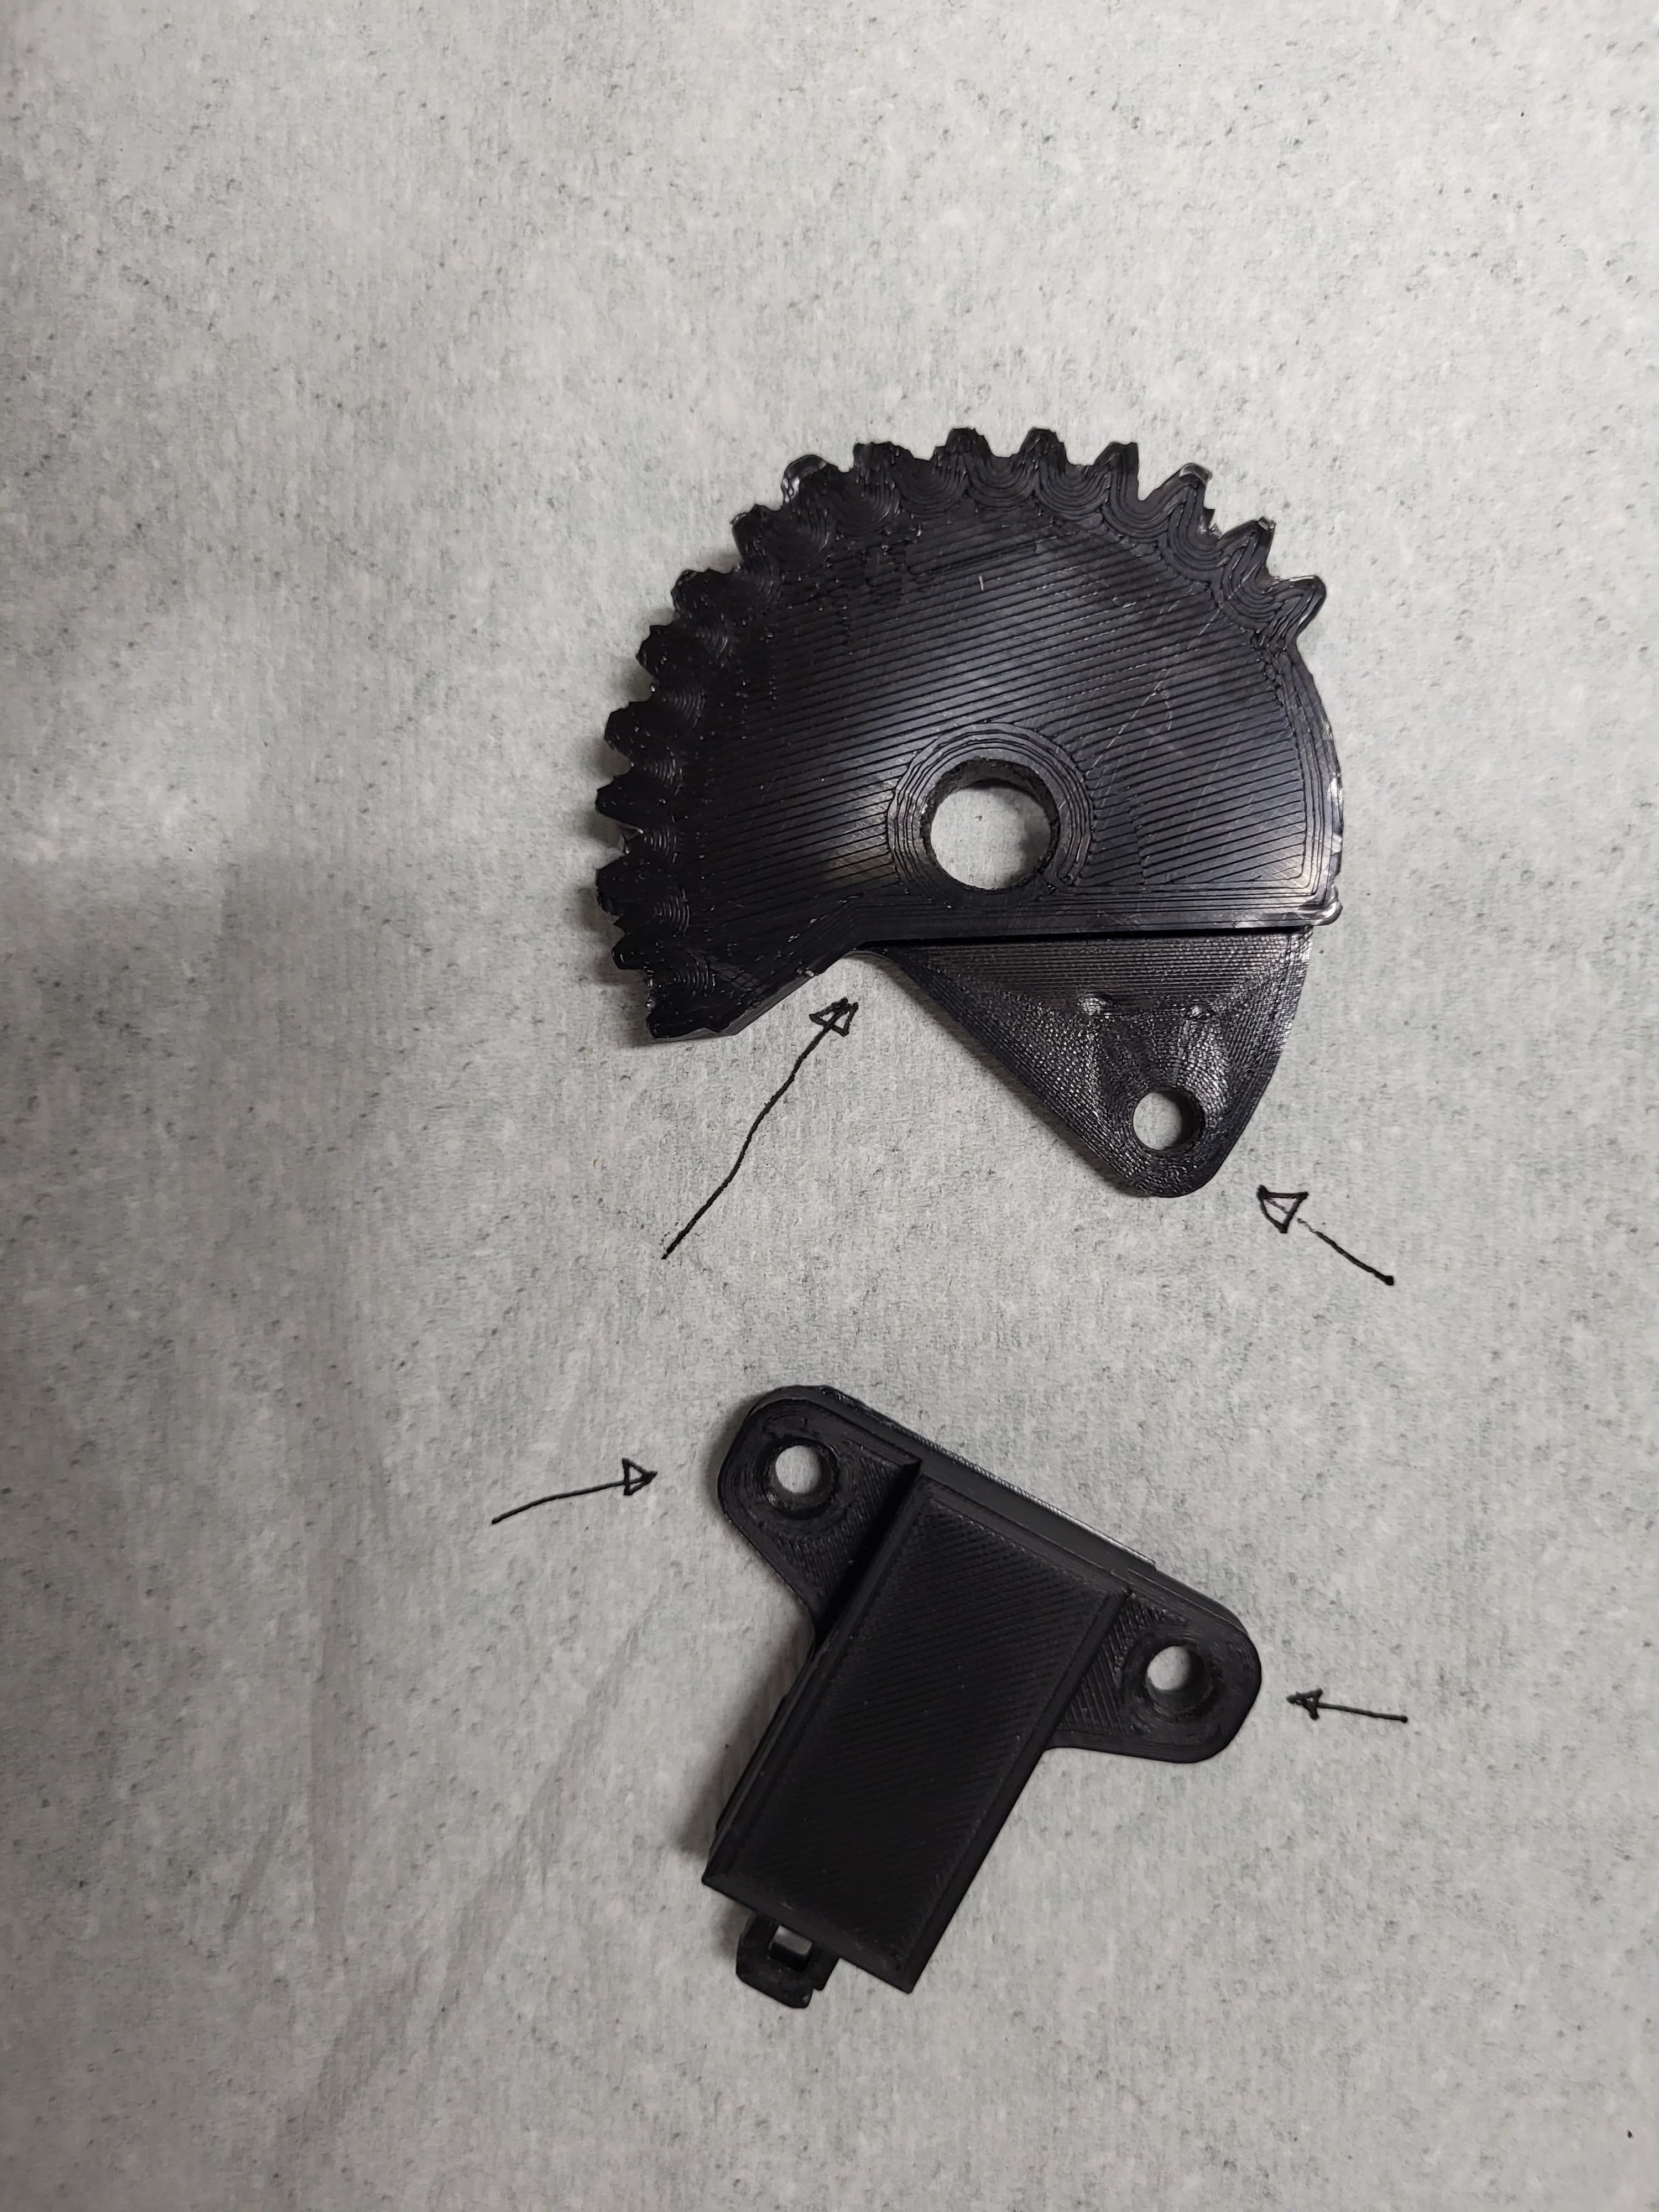
\includegraphics[height=9cm]{img/greifarmtest/prototyp_test_loecher.jpeg}
        \caption{Schrumpfungseffekte 3D-Druck: Alle Löcher sind zu klein}
        \label{fig:hardware_test_loecher}
    \end{minipage}%
    \hfill
    \begin{minipage}[t]{0.45\textwidth}
        \centering
        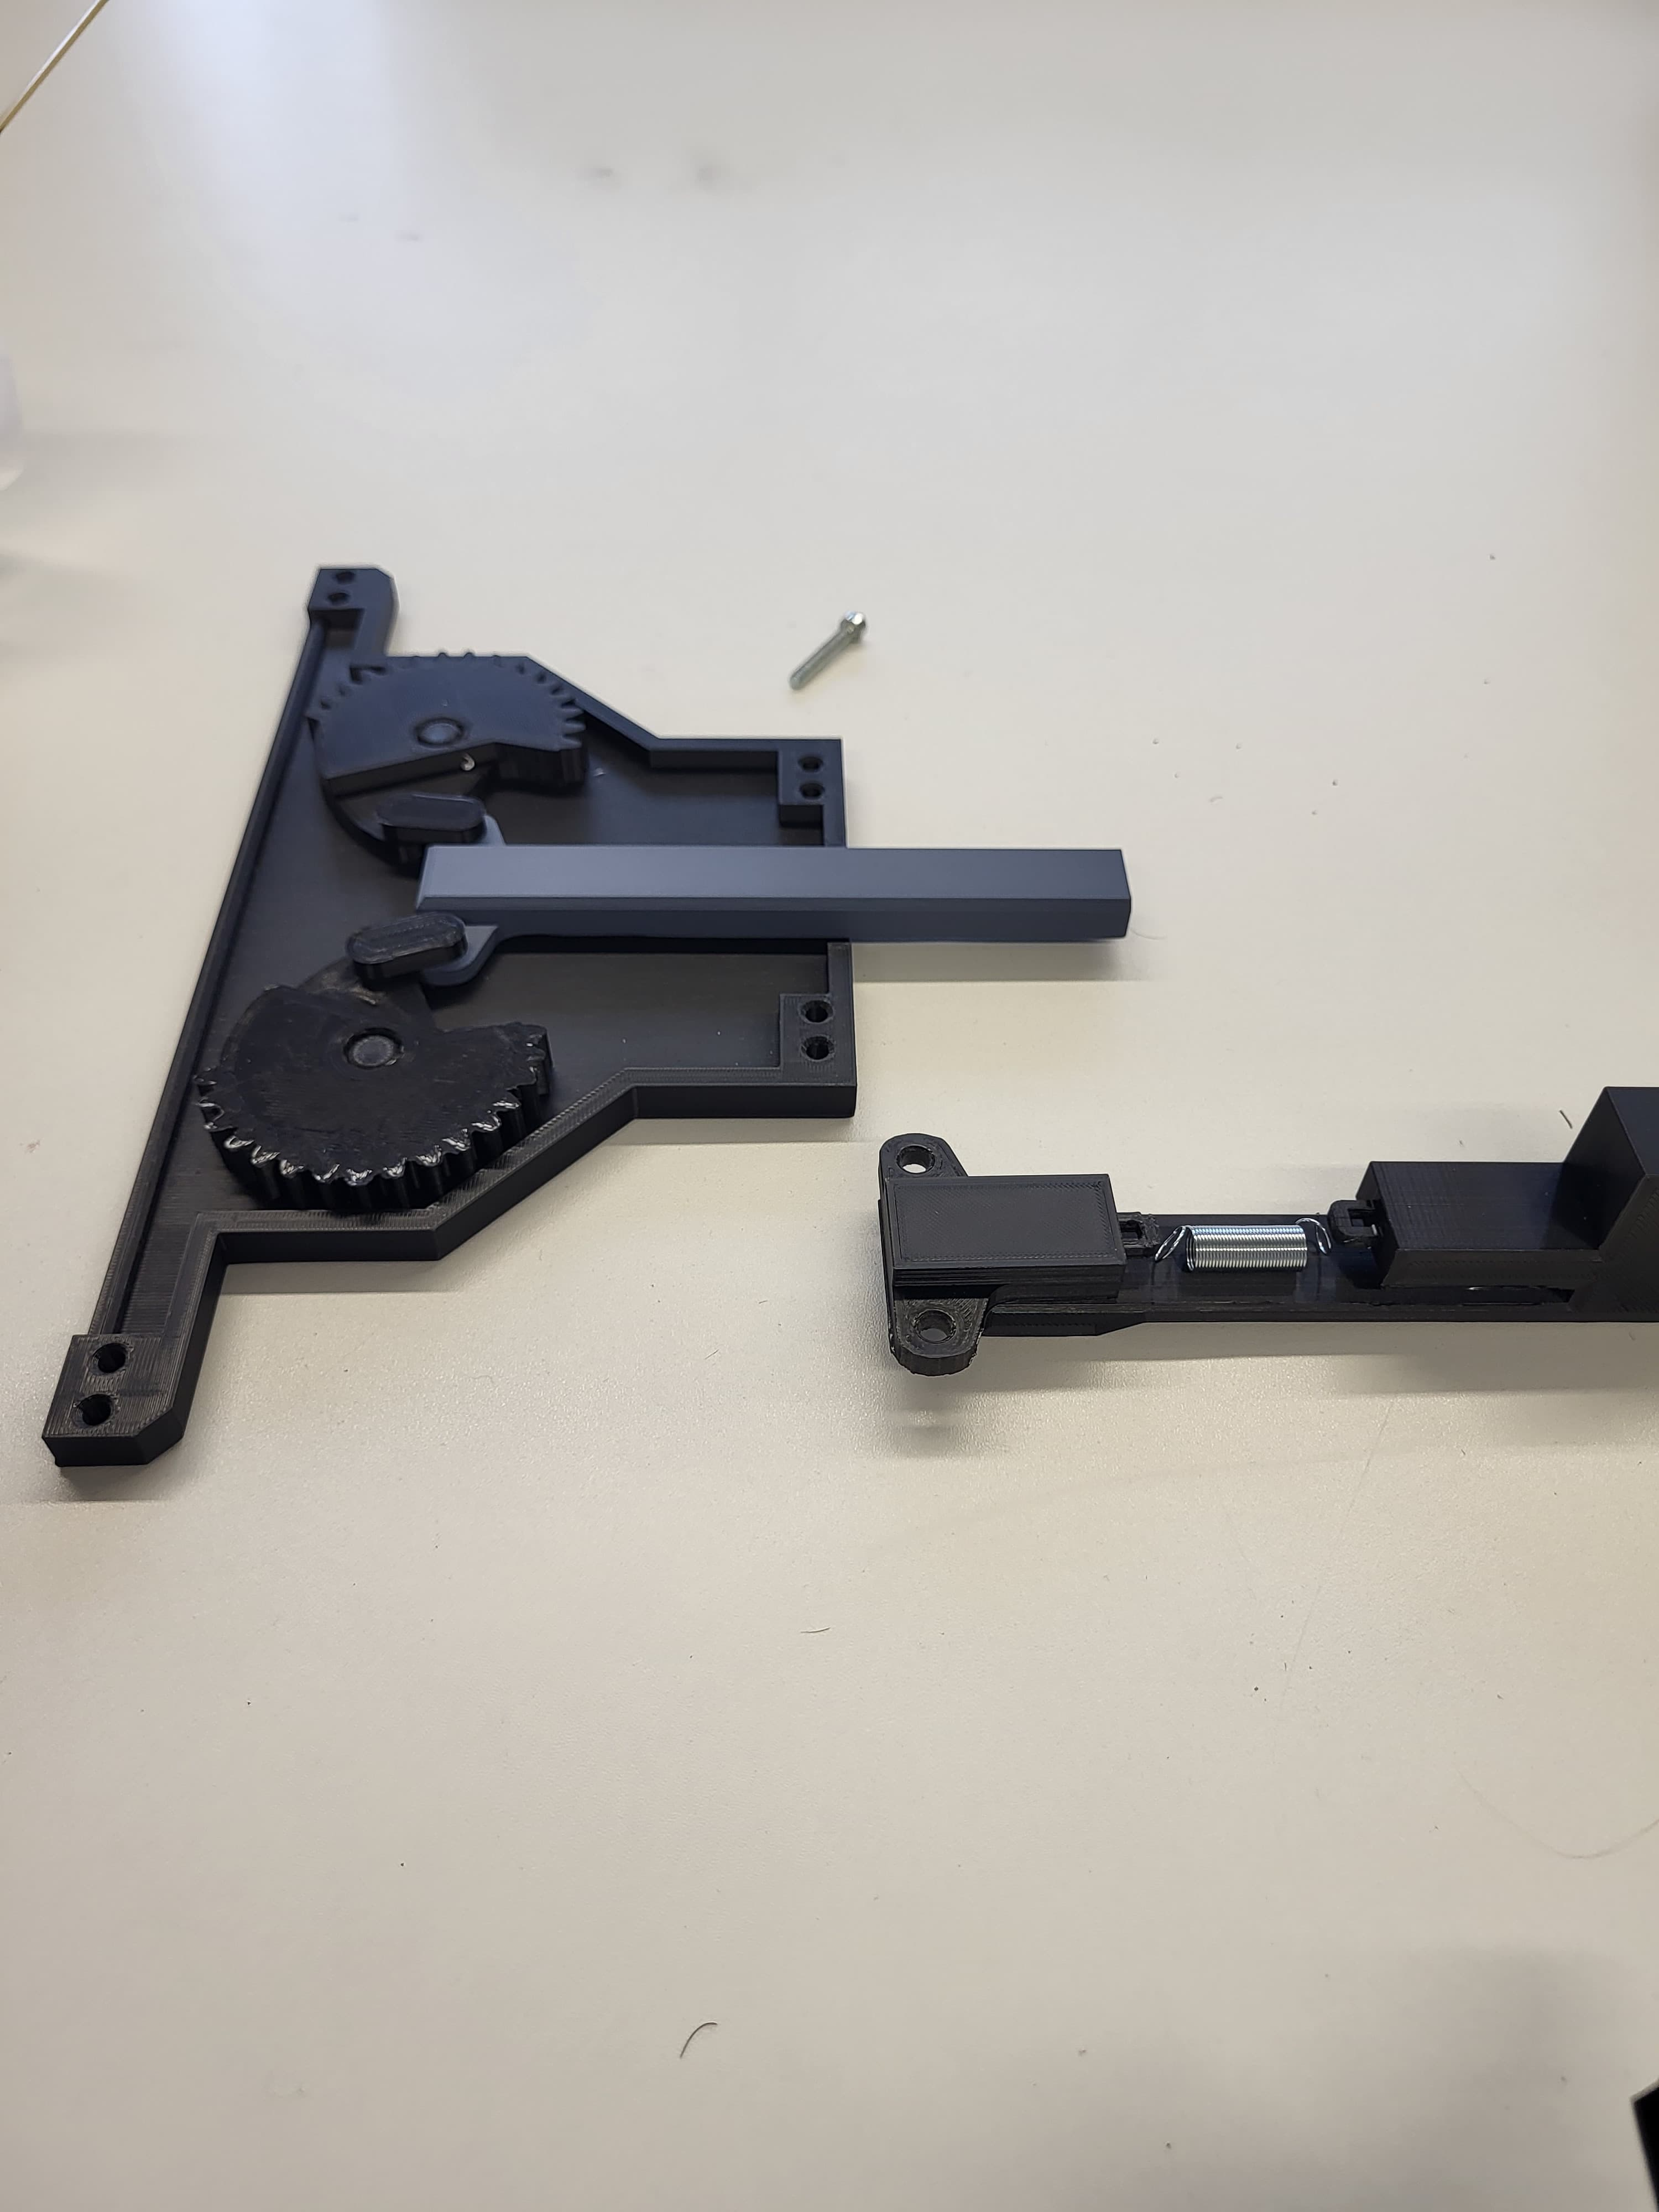
\includegraphics[height=9cm]{img/greifarmtest/prototyp_test_schieber.jpeg}
        \caption{Feder wurde temporär durch einen Schieber ersetzt.}
        \label{fig:hardware_test_schieber}
    \end{minipage}
\end{figure}
\newpage
\subsubsection{Distanzmessung Hindernis}
Für die Positionierung der Klemmbacken um das Hindernis ist eine Abstandsmessung erforderlich. Im Rahmen der Technologierecherche (siehe Anhang \ref{technologierecherche}) wurden hierfür ein Ultraschallsensor und ein \acrshort{tof-sensor} identifiziert. Der Ultraschallsensor wurde gewählt, da er auch bei direkter Sonneneinstrahlung konstante Messwerte liefert. Die durchgeführten Tests zeigten stabile Messungen ab einem Mindestabstand von 3 cm und einer getesteten Reichweite von 30 cm. Der Mindestabstand von 3 cm ist bei der Installation zu berücksichtigen. Der genaue Versuchsaufbau sowie die Messergebnisse sind im Anhang \ref{sec:Distanz_Hindernis} detailliert beschrieben.

\subsubsection{Linienerkennung / Punkterkennung}
Um der Linie zu folgen und den Punkt zu erkennen, ist ein geeigneter Sensor erforderlich. In der Technologierecherche (siehe Anhang \ref{technologierecherche}) wurden zwei mögliche Sensoren identifiziert: ein Farbsensor und ein \gls{ir-fototransistor}. Obwohl der Farbsensor zuverlässig Unterschiede zwischen Boden und Linie erkennt, schied er aufgrund seiner relativ langen Belichtungszeit von 100 ms aus. Er liefert nur alle 100 ms einen Messwert, was bei einer Geschwindigkeit von 20 cm/s nur eine Abtastrate von einem Messwert pro 2 cm ergibt und damit nicht ausreicht.

Der \gls{ir-fototransistor} hingegen liefert Messwerte alle 2 ms und erkennt auch deutlich die Unterschiede zwischen den verschiedenen Oberflächen. Darüber hinaus ermöglicht die Analyse der Strichdicke mit mehreren IR-Fototransistoren eine genaue Punkterkennung. Die Details der Versuche und Ergebnisse sind im Anhang \ref{a4:Infrarot-Fototransistor-Array} dokumentiert.
Das Schema und Layout für den Liniensensor, der mit IR-Dioden und IR-Fototransistoren arbeitet, wurde bereits erstellt (siehe Anhang \ref{a5:Schema-Linefollower}).
\end{document}